% Chapter Template

\chapter{Large Hadron Collider} % Main chapter title

\label{Chapter3} % Change X to a consecutive number; for referencing this chapter elsewhere, use \ref{ChapterX}

\lhead{Chapter 3. \emph{Large Hadron Collider}} % Change X to a consecutive number; this is for the header on each page - perhaps a shortened title


Physics goals go here.

%----------------------------------------------------------------------------------------
%	SECTION 1
%----------------------------------------------------------------------------------------

\section{Design of the Large Hadron Collider}


\begin{figure}[htbp]
	\centering
		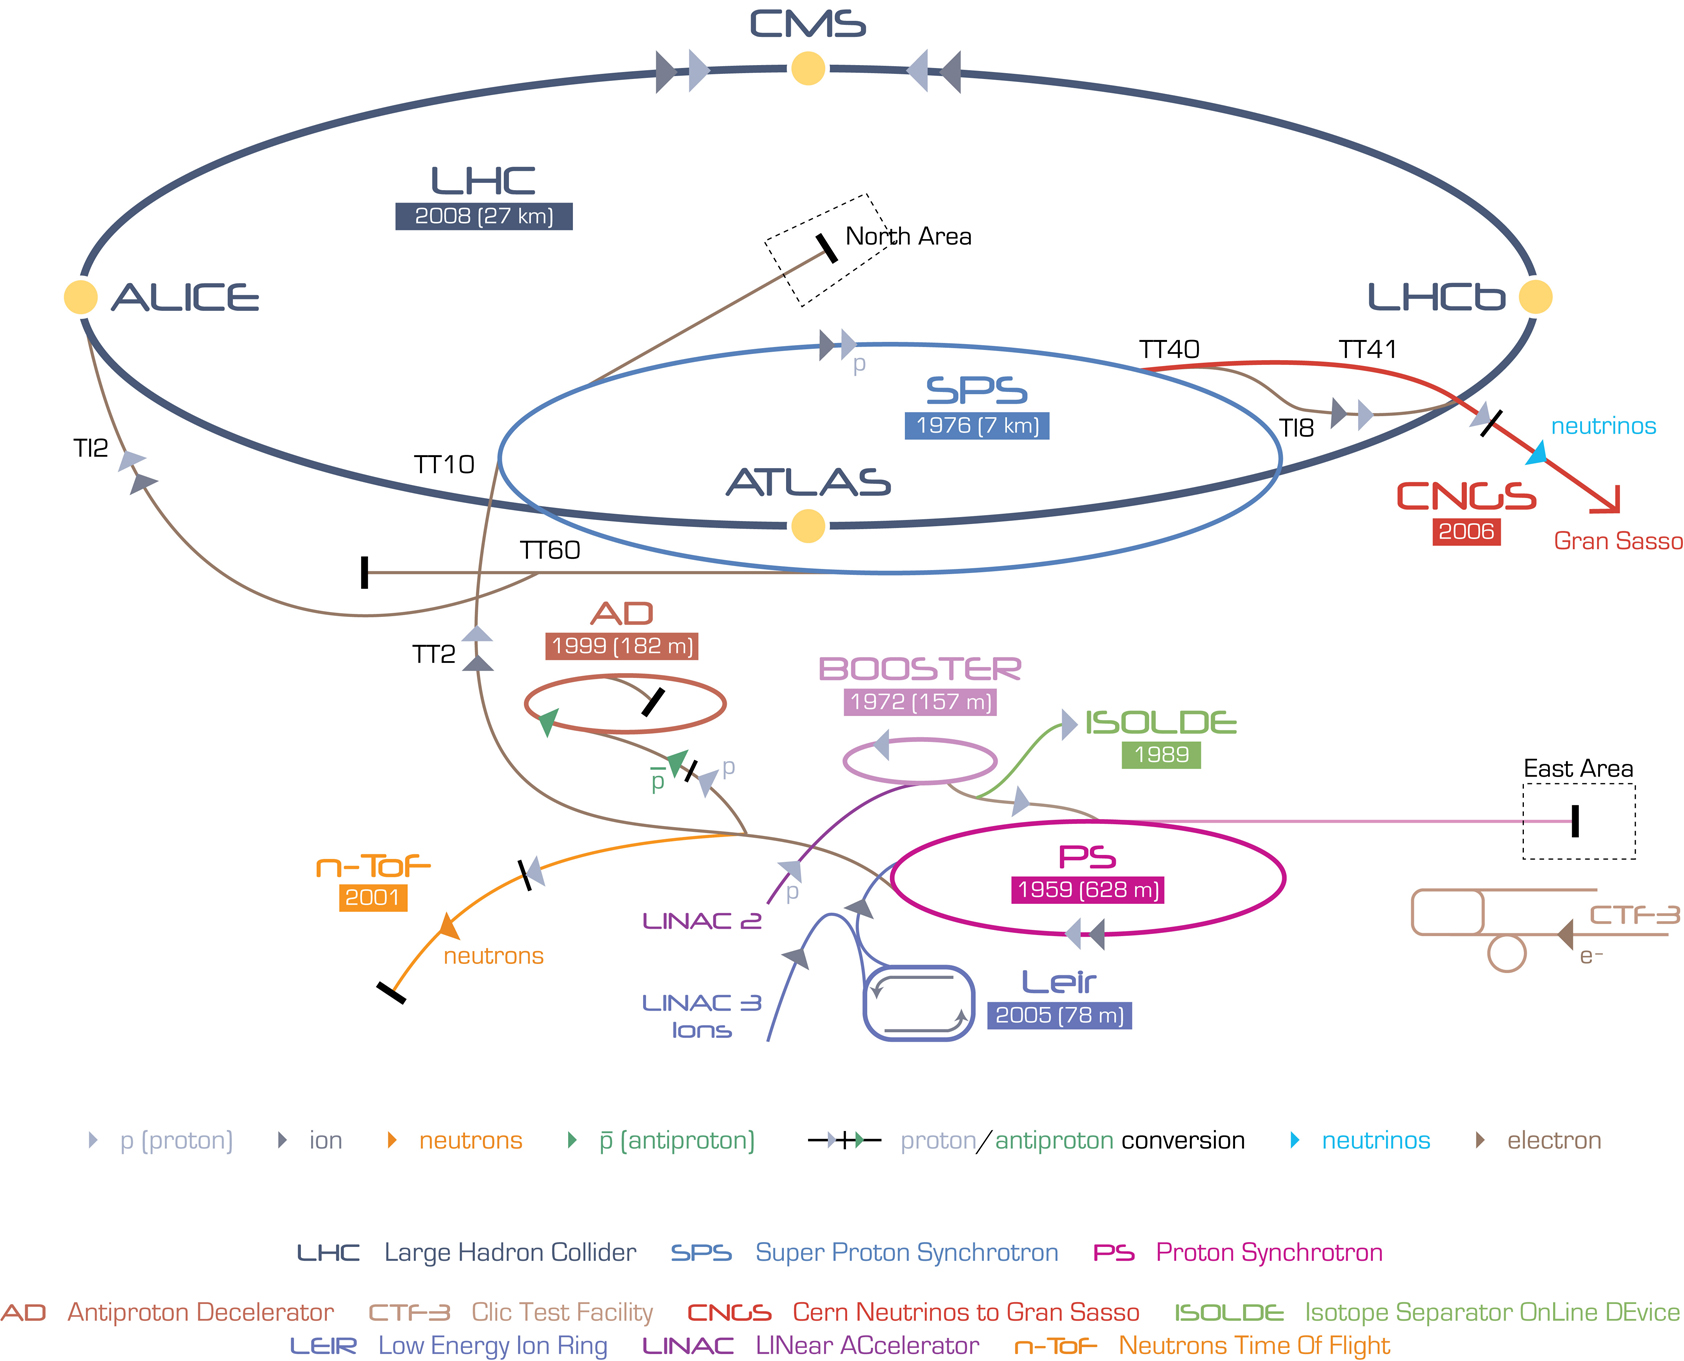
\includegraphics[width=0.9\textwidth]{Figures/LHC.jpg}
		%\rule{35em}{0.5pt}
	\caption[Schematics of Large Hadron Collider]{Schematics of Large Hadron Collider}
	\label{fig:LHC}
\end{figure}

\begin{figure}[htbp]
	\centering
		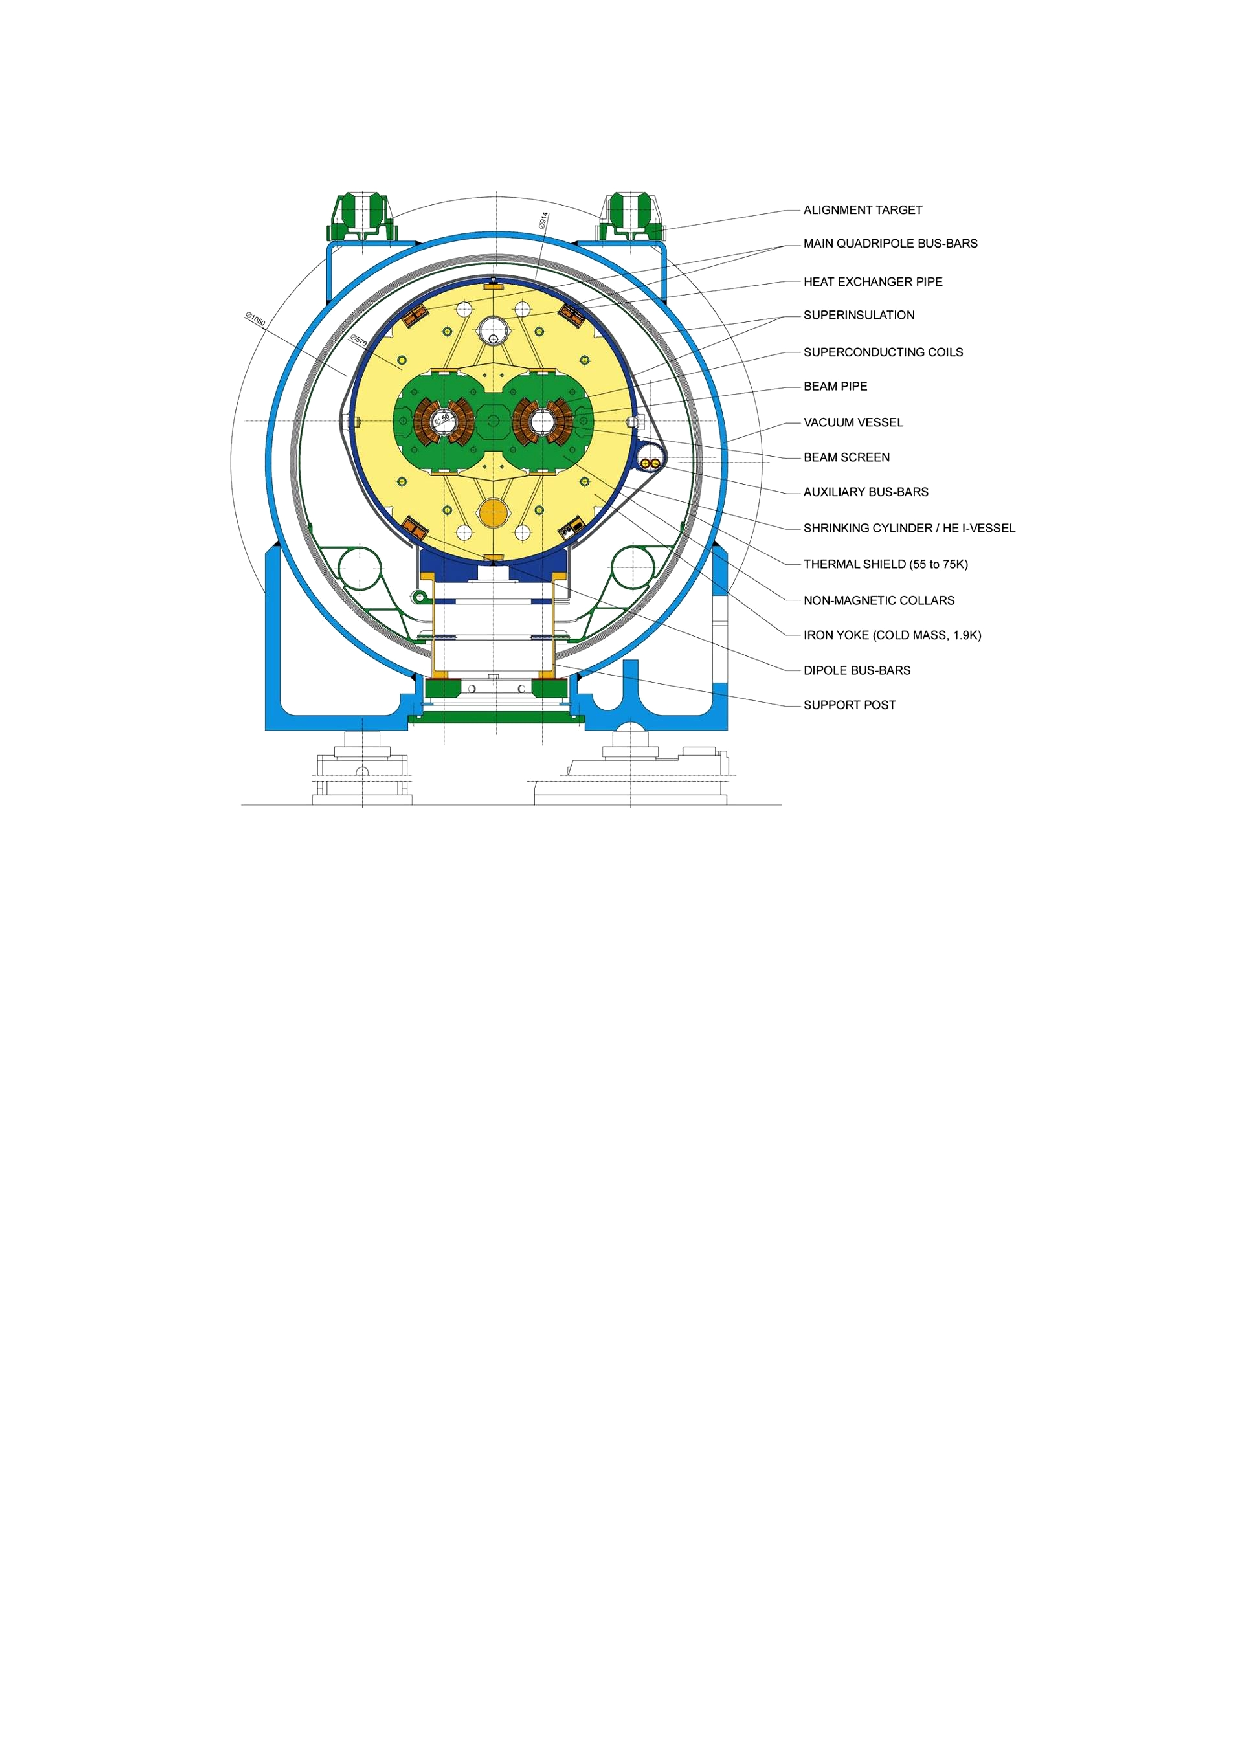
\includegraphics[width=0.9\textwidth]{Figures/LHC_magnet.pdf}
		%\rule{35em}{0.5pt}
	\caption[Schematics of dipole magnets]{Schematics of Dipole magnets}
	\label{fig:LHC_mag}
\end{figure}

%-----------------------------------
%	SECTION 2
%-----------------------------------

\section{Performance}
